\section{Продвинутые подходы автоматизации тестирования} 

До настоящего момента под <<автоматизацией>> понималась автоматизация выполнения тестов. Продвинутые подходы к автоматизации тестирования расширяют понятие атоматизиции. Они исключают человеческий фактор в процессе тестирования. Это означает отсутсвие необходимости разрабатывать тестовые сценарии. Компьютер сделает это за человека. Иногда такие подходы называются тестированием с помощью искусственного интелекта.

\subsection{Статическое тестирование} 

Статическое тестирование (статический анализ)~--- автоматизированный процесс ревизии кода без его исполнения. Статическое тестирование позволяет быстро найти ошибки низкой и средней сложности (использование неактуальной библиотеки, обращение к пустому указателю и т.~д.). Распространенные инструменты статического анализа: \textit{PMD, Checkstyle, Checkmarx}.

Классический подход к статическому анализу заключается в проверке исходного кода системы на потенциальные структурные или стилистические уязвимости. Анализатор состоит из парсера и набора правил. Существуют две техники статического анализа:


\begin{enumerate}
	\item Сопоставление с образцом с помощью регулярных выражений.
	\item Синтаксический анализ абстрактного ситаксического дерева.
\end{enumerate}


\subsubsection{Сопоставление с образцом}

Сопоставление с образцом~--- проверка кода, входе которой происходит поиск соответствия заданному ранее образцу. Образец задается с помощью \textbf{регулярного выражения}. Регулярное выражение~--- последовательность символов, представляющая образец.

Недостатком сопоставления с образцом является отсутствие контекта исполнения. Другими словами, сопоставление с образцом не учитывает семантику программы. Например, задав регулярное выражение \texttt{$\textbackslash$s*System.out.println\textbackslash(.*\textbackslash);} сопоставление с образцом определит 3 строки в листинге~1.17. Из чего можно сделать вывод, что программа напечатает 3 раза некоторое сообщение. Однако, программа не напечатает ни одного сообщения. 

\begin{ListingEnv}[!h]% настройки floating аналогичны окружению figure
	\captiondelim{ } % разделитель идентификатора с номером от наименования
	\caption{Пример неучитанной семантики}
	% окружение учитывает пробелы и табуляции и применяет их в сответсвии с настройками
	\begin{lstlisting}[language={Java}]
boolean DEBUG = false;

if (DEBUG){
	System.out.println("Debug line 1");
	System.out.println("Debug line 2");
	System.out.println("Debug line 3");
}
	\end{lstlisting}
\end{ListingEnv}%


\subsubsection{Синтаксический анализ}

Более продвинутый способ анализа кода~--- синтаксический анализ. В ходе синтаксического анализа текст программы разбивается на поток символов, символы пребразубтся в токены, а из токенов составляется \textit{дерево разбора}. Дераво разбора представляет собой синтаксическое дерево конкретной версии кода. В синтаксическом анализе используется \textit{абстрактое синтаксическое дерево}~--- дерево разбора без синтаксических деталей (точки с запятой, скобки). Пример абстрактного синтаксического дерева кода из листинга~1.17 представлен на рис.~\ref{img:ast}

\begin{figure}[ht]
	\centering
	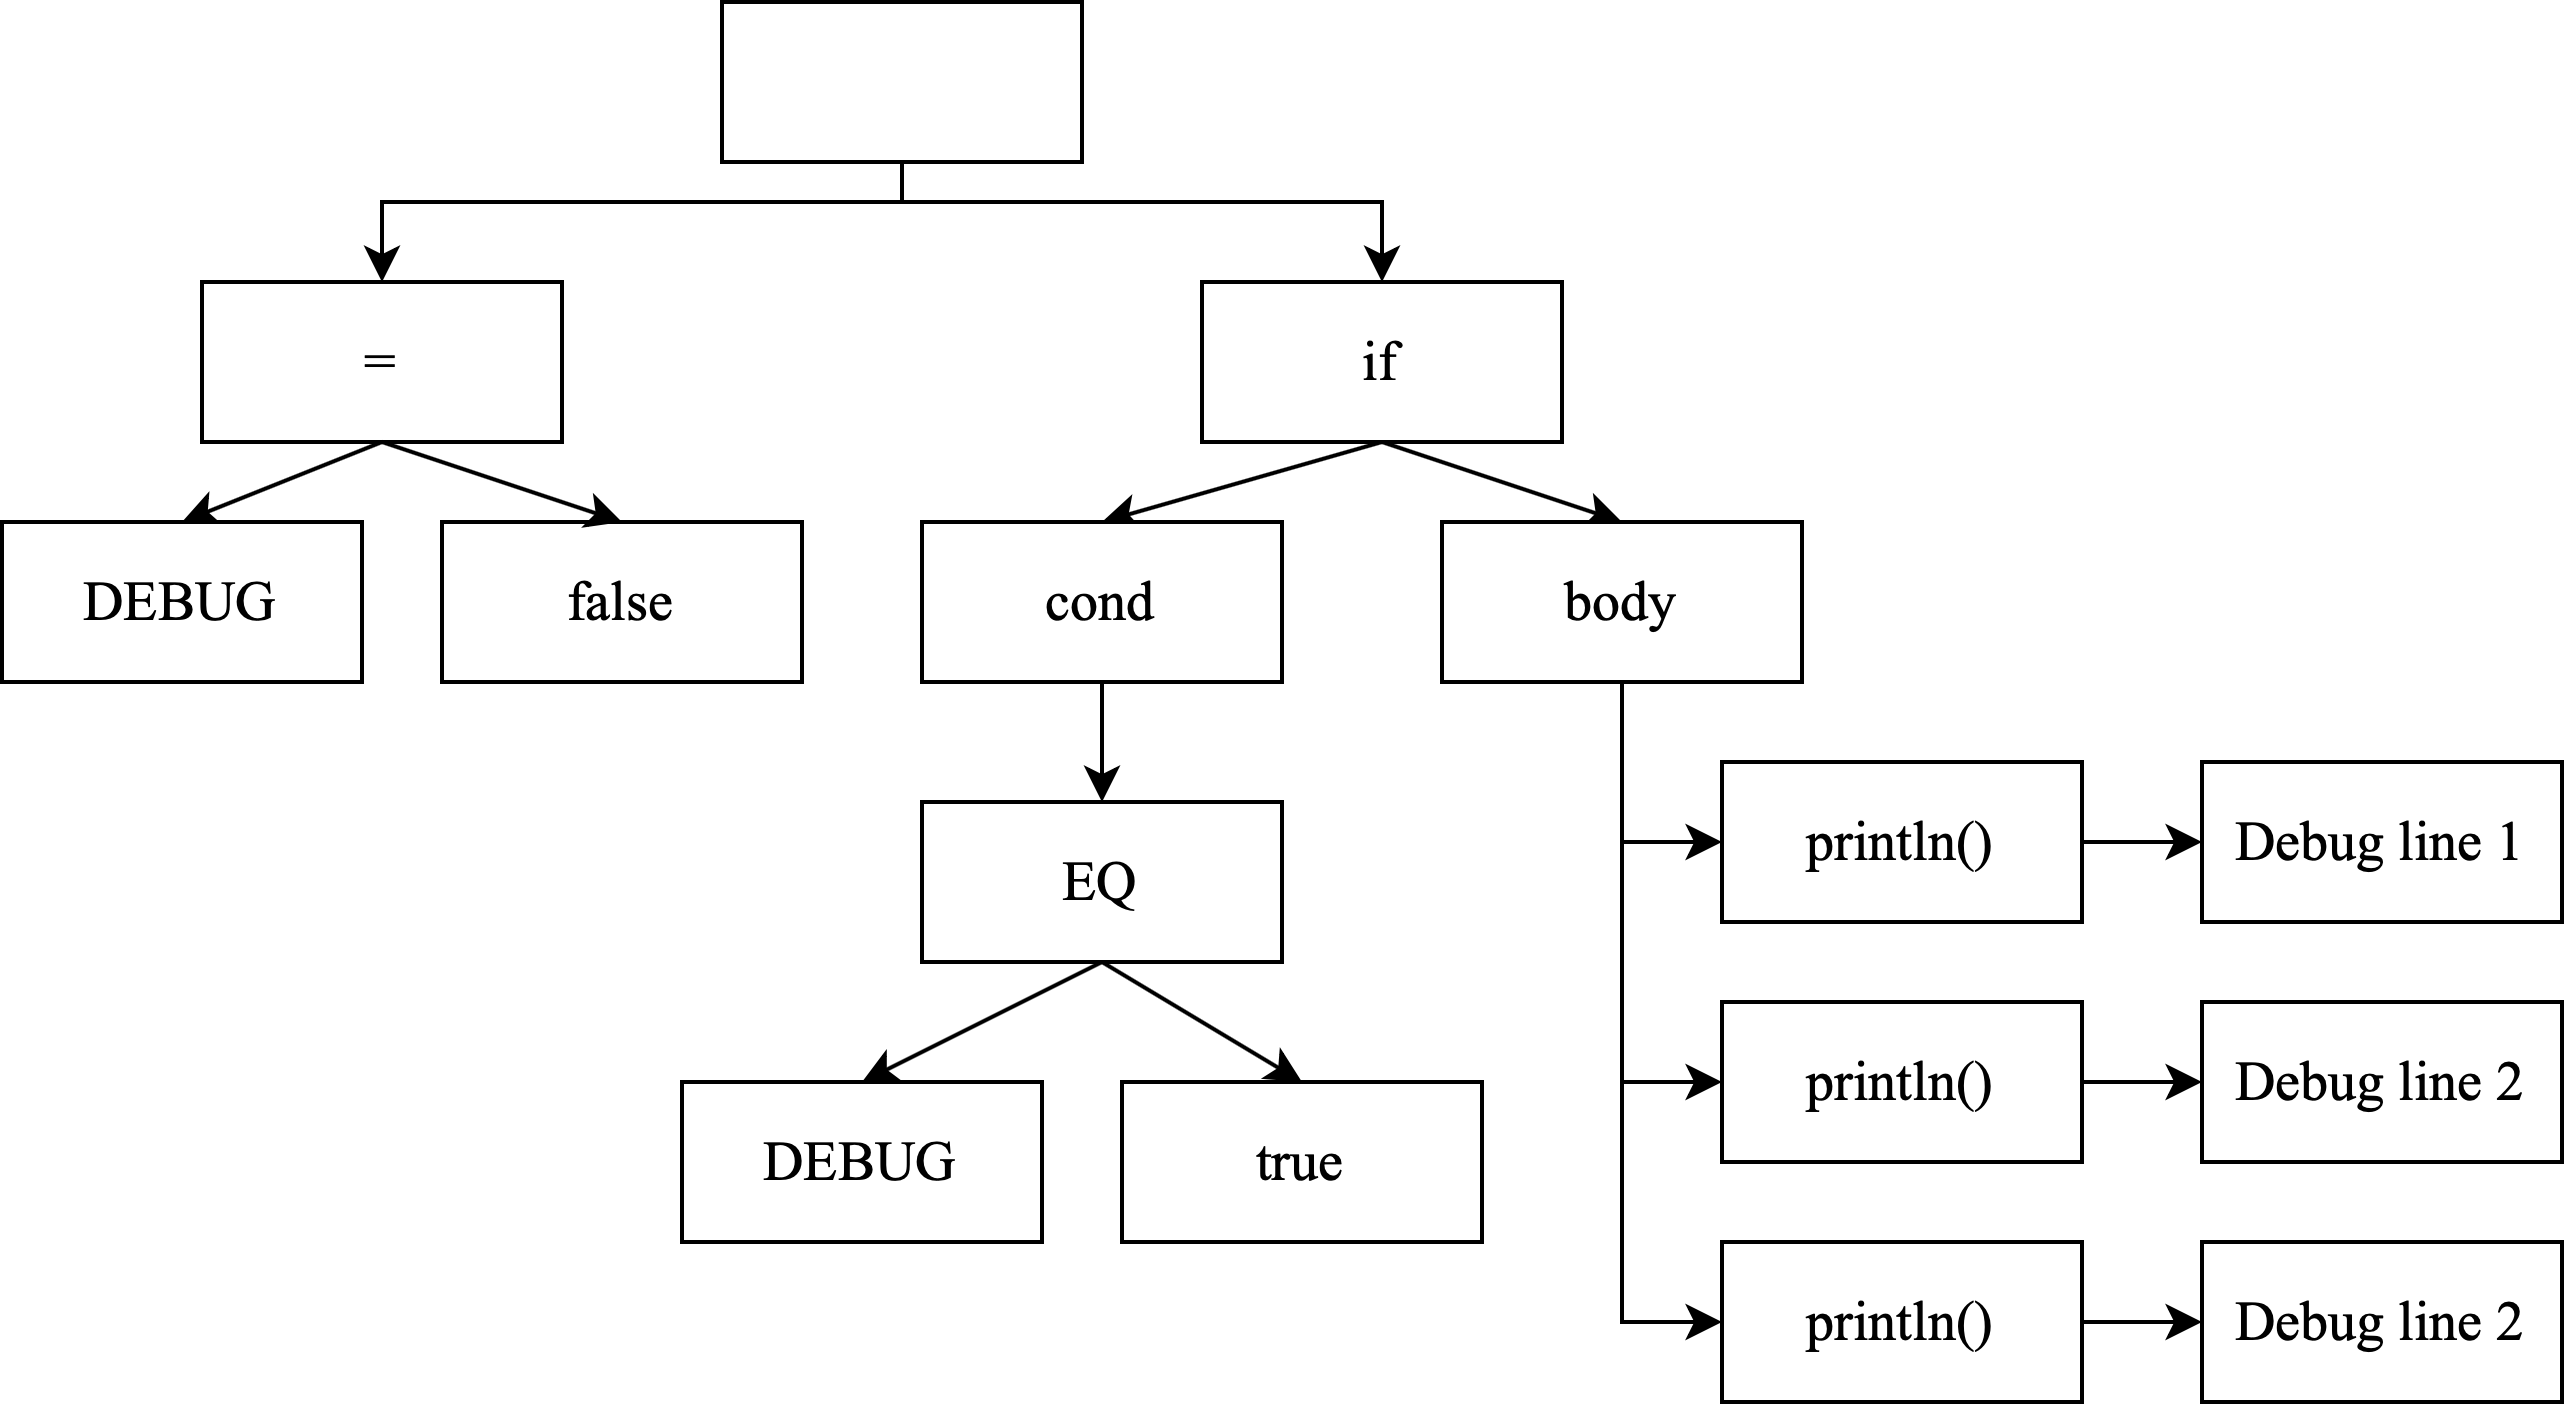
\includegraphics [scale=0.9] {AST_TR}
	\caption{Абстрактное синтаксическое дерево}
	\label{img:ast}
\end{figure}


Статический анализатор, использующий ситаксический анализ, принимает на вход абстрактное синтаксическое дерево и набор правил. Анализатор сообщает о найденных несоответствиях в коде.


\subsection{Мутационное тестирование} 
 
  \fixme{TBD}
 

\subsection{Генерация входных данных} 
 
 \fixme{TBD}
 

\subsection{Тестирование на основе анализа кода} 
 
 \fixme{TBD}
 
